\subsection{Descripció de les funcionalitats}

    \paragraph{}
    Les funcionalitats d'identificació i desconnexió a l'API de FamilySearch, s'utilitzen exactament pel que el seu nom indica, per permetre als usuaris identificar-se o desconnectar-se de FamilySearch, des de la pàgina d'un tercer.

    Els usuaris no disposen de permisos d'interacció amb l'API, a menys que s'identifiquin primer en el sistema. El motiu, és que un cop identificats, cada usuari rep un `token', que al ser adjuntat a les crides a l'API, fa que aquestes siguin acceptades.

    En l'aplicació web implementada, la possibilitat d'identificar-se amb FamilySearch apareix quan l'usuari intenta accedir a la secció d'exemples o a un exemple concret. La pàgina en qüestió és relativament simple. L'usuari disposa de dues opcions, tornar enredera o identificar-se amb FamilySearch.

    La figura~\ref{fig:fsLogin} mostra la pàgina d'identificació.

    \begin{figure}
        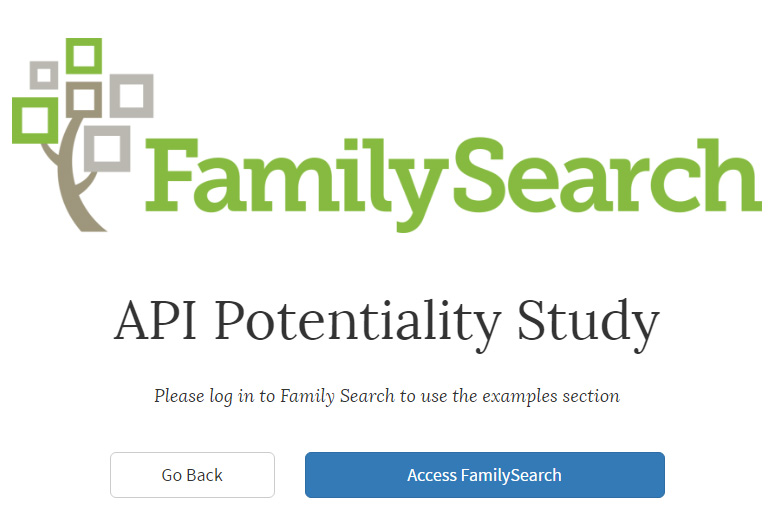
\includegraphics[scale=0.4]{11/01_loginLogout/01_loginImage}
        \centering
        \caption{Pàgina d'identificació}\label{fig:fsLogin}
    \end{figure}

    Un cop els usuaris es troben identificats, tenen l'opció de desconnectar-se, des de qualsevol pàgina del web, mitjançant un botó situat a la part dreta de la barra de navegació.
